\documentclass[11pt,a4paper]{article}
\usepackage[T1]{fontenc}
\usepackage[margin=2.3cm]{geometry}
\usepackage{amsmath,amssymb}
\usepackage{booktabs}
\usepackage{graphicx}
\usepackage{xcolor}
\usepackage{enumitem}
\usepackage{tcolorbox}
\usepackage{hyperref}
\usepackage{multirow}
\graphicspath{{../report/figures/}{../presentation/extra_figures/}}
\hypersetup{colorlinks=true, linkcolor=blue!60!black, urlcolor=blue!60!black}
\setlist{nosep}
\newtcolorbox{qa}[1]{colback=blue!4, colframe=blue!50!black, title={#1}, fonttitle=\bfseries, left=4pt, right=4pt, top=3pt, bottom=3pt}
\newtcolorbox{key}{colback=orange!8, colframe=orange!70!black, left=4pt, right=4pt, top=3pt, bottom=3pt}
\newcommand{\yhat}{\hat{y}}

\title{\textbf{Viva Preparation Guide}\\[4pt]\Large Auditing Fairness and Bias in Classical ML Income Prediction}
\author{Group 17 --- Saransh Gupta, Sayan Samajpati, Ayush Anand, Adabala Sridhar\\\small Indian Institute of Information Technology, Allahabad}
\date{November 2026}

\begin{document}
\maketitle

\begin{key}
\textbf{How to use this guide.} It explains, in order, every idea and every step in our project so that any team member can defend any part of it. Boxes marked \emph{Q} are questions an examiner is likely to ask, with model answers. All numbers are the real ones from \texttt{experiments/results/} and match the report. Read the whole thing once; then re-read Sections~\ref{sec:story}, \ref{sec:results} and \ref{sec:questions} the night before.
\end{key}

\tableofcontents
\newpage

%====================================================================
\section{The project in one page}\label{sec:story}

\textbf{Question we ask.} Models that predict income (or creditworthiness) are evaluated by accuracy. Accuracy is one number for everybody. Does a model that is ``87\% accurate'' treat men and women, or different races and ages, the same way? If not, how big is the difference, is it real, and can we fix it?

\textbf{What we did.}
\begin{enumerate}
  \item Took the \textbf{UCI Adult} dataset (48,842 adults from the 1994 US census). Label: does the person earn more than \$50K a year? Yes for 23.9\%.
  \item Cleaned it, split it into train / validation / test (60 / 15 / 25\%).
  \item Trained four \textbf{classical} models: logistic regression, linear SVM, random forest, gradient boosting. Each twice: with and without the columns \texttt{sex} and \texttt{race}.
  \item \textbf{Audited} every model: for each group (men/women, each race, each age band, sex$\times$race) we measured how often the model says ``$>$50K'', how often it finds the true high earners, how often it wrongly flags low earners, and how reliable a positive prediction is.
  \item Checked the gaps are \textbf{statistically significant} (bootstrap confidence intervals, $z$-test, $\chi^2$ test).
  \item Applied \textbf{five bias-mitigation methods} (pre-, in- and post-processing) and measured what each buys and what it costs.
\end{enumerate}

\textbf{What we found.}
\begin{itemize}
  \item Best model: gradient boosting, 87.0\% accuracy, F1 0.707, AUC 0.925.
  \item It predicts ``$>$50K'' for \textbf{26.4\% of men vs 8.3\% of women} (demographic parity gap 0.181). Among people who really earn $>$50K it finds 66.8\% of men but 57.7\% of women (equal opportunity gap 0.091). $p<10^{-10}$: not noise.
  \item Per-group \emph{accuracy} is higher for women (93.3\% vs 83.9\%) --- which is misleading; it only means fewer women are positive. This is why accuracy alone hides bias.
  \item \textbf{Removing sex and race does not help} (gap 0.171): marital status, relationship, occupation, hours act as proxies.
  \item Changing the algorithm does not help either (DP gap 0.159--0.181 across all 8 models): the bias is in the data.
  \item Age gives the largest gap (0.321), intersectional groups (Asian-Pac-Islander men vs Black women) 0.312.
  \item Mitigation works but each method fixes one criterion and often worsens another: reweighing $\to$ DP 0.101 ($-0.6$ accuracy points); group thresholds $\to$ EO 0.002 ($-0.2$); equalized-odds post-processing and in-processing reach the smallest gaps but cost 1--2.4 points and destroy predictive parity. There is no free lunch.
\end{itemize}

%====================================================================
\section{The dataset}

\subsection{Facts to remember}
\begin{itemize}
  \item \textbf{Name:} UCI Adult / Census Income. Source: UCI Machine Learning Repository; we load it from OpenML (\texttt{fetch\_openml("adult", version=2)}). Extracted by Kohavi (1996) from the 1994 US census.
  \item \textbf{Size:} 48,842 rows, 14 attributes + label. After dropping 52 exact duplicates: 48,790 rows.
  \item \textbf{Label:} \texttt{class} $\in\{\leq$50K, $>$50K$\}$; we code $y=1$ for $>$50K. 23.9\% positive $\Rightarrow$ class imbalance.
  \item \textbf{Features used (13):} age, workclass, education, education-num, marital-status, occupation, relationship, race, sex, capital-gain, capital-loss, hours-per-week, native-country.
  \item \textbf{Dropped:} \texttt{fnlwgt} (``final weight'': how many people in the population a row represents --- a survey artefact, not a property of the person).
  \item \textbf{Missing values:} written as ``?'' in the original (already NaN in the OpenML copy): workclass 2,795, occupation 2,805, native-country 856.
  \item \textbf{Sensitive attributes:} sex (Male 66.8\%, Female 33.2\%), race (White 85.5\%, Black 9.6\%, Asian-Pac-Islander 3.1\%, Amer-Indian-Eskimo 1.0\%, Other 0.8\%), and age group (<30, 30--44, 45--59, 60+) which we derived from age.
  \item \textbf{Bias is already in the labels:} 30.4\% of men vs 10.9\% of women earn $>$50K; 5.4\% of under-30s vs 38.8\% of 45--59.
\end{itemize}

\subsection{Cleaning and preprocessing}
\begin{itemize}
  \item Strip whitespace, convert ``?'' to NaN, drop duplicate rows, drop \texttt{fnlwgt}.
  \item \textbf{Imputation:} numeric columns $\to$ median, categorical $\to$ most frequent value.
  \item \textbf{Scaling:} numeric columns standardized (zero mean, unit variance). Needed for logistic regression and SVM; harmless for trees.
  \item \textbf{Encoding:} categorical columns one-hot encoded (\texttt{handle\_unknown="ignore"}). Result: 104 input columns with sex/race, 97 without.
  \item All of this lives inside a scikit-learn \texttt{Pipeline} with a \texttt{ColumnTransformer}, \textbf{fitted on the training split only}.
\end{itemize}

\begin{qa}{Q: Why put preprocessing inside the pipeline instead of doing it once on the whole table?}
To avoid \textbf{data leakage}. If the median or the scaler's mean were computed on all rows, information from the test set would influence the model. The pipeline fits the imputer/scaler/encoder on training data and only \emph{applies} them to validation and test data, exactly as would happen in deployment.
\end{qa}

\begin{qa}{Q: Why drop \texttt{fnlwgt}?}
It is a census sampling weight (how many US residents a record stands for). It carries no information about the individual and would be meaningless at prediction time for a new person.
\end{qa}

\subsection{The split}
25\% is held out first as the \textbf{test set} (12,198 rows). The remaining 75\% is split 80/20 into \textbf{training} (29,273 rows, 60\%) and \textbf{validation} (7,319 rows, 15\%). Stratified on the label so every split has 23.9\% positives. Random seed 42 everywhere.

\begin{itemize}
  \item \textbf{Training:} fitting the models and 3-fold cross-validation for hyperparameters.
  \item \textbf{Validation:} recording the loss curves, choosing the group-specific thresholds and fitting the equalized-odds post-processor.
  \item \textbf{Test:} touched once per final model; every number in the report is a test-set number.
\end{itemize}
Test set group sizes: 8,194 men / 4,004 women; 10,459 White, 1,152 Black, 367 Asian-Pac-Islander, 116 Amer-Indian-Eskimo, 104 Other; age 3,607 / 4,688 / 2,864 / 1,039.

\begin{qa}{Q: Why stratify? Why a validation set if you already use cross-validation?}
Stratifying keeps the 24/76 class ratio in every split so metrics are comparable. Cross-validation on the training set picks hyperparameters; the separate validation set is needed for things that must be fitted \emph{after} the model is final but \emph{before} we look at test data: the loss-vs-epoch curves and the post-processing rules (thresholds). Choosing thresholds on the test set would be cheating.
\end{qa}

%====================================================================
\section{The models}

All four are classical (no neural networks), from scikit-learn 1.9.1. Each is tuned by \textbf{grid search with 3-fold stratified cross-validation on the training split, maximizing F1} (because the classes are imbalanced, F1 is more informative than accuracy).

\begin{center}\footnotesize
\begin{tabular}{p{2.3cm}p{5.2cm}p{4.3cm}p{2.2cm}}
\toprule
Model & How it works (one line) & Grid & Chosen \\
\midrule
Logistic regression & linear model, sigmoid of a weighted sum, $\ell_2$ penalty & $C\in\{0.01,0.1,1,10\}$ & $C$=10 / 1 \\
Linear SVM & linear boundary maximizing the margin (hinge loss) & $C\in\{0.01,0.1,1\}$ & $C$=1 \\
Random forest & 200 decision trees on bootstrap samples, majority vote & depth $\{10,20,\infty\}$, min leaf $\{1,5\}$ & depth 20, leaf 1 \\
Gradient boosting & trees fitted sequentially to the residual (gradient of log loss) & lr $\{0.05,0.1\}$, iters $\{200,400\}$, leaves $\{15,31\}$ & 0.1, 200, 31 \\
\bottomrule
\end{tabular}
\end{center}

\begin{qa}{Q: What is $C$ in logistic regression / SVM?}
Inverse regularization strength. Small $C$ = strong regularization = simpler model (weights shrunk towards zero). Large $C$ = fits training data more closely. We tried 0.01 to 10 and picked by cross-validated F1.
\end{qa}

\begin{qa}{Q: Why \texttt{HistGradientBoostingClassifier} rather than \texttt{GradientBoostingClassifier}?}
It bins continuous features into histograms (255 bins) so each tree is built much faster on 30k rows; it is scikit-learn's LightGBM-style implementation. Same idea: boosting of shallow trees on the log-loss gradient.
\end{qa}

\begin{qa}{Q: Why a \emph{linear} SVM and not RBF?}
An RBF kernel SVM on 30k rows $\times$ 100 features is slow (quadratic in the number of samples) and the project rules say keep everything runnable on free Colab. LinearSVC uses liblinear and trains in under a second. Its accuracy equals logistic regression here (85.2\%), so nothing was lost.
\end{qa}

\subsection{Performance (test set)}
\begin{center}\small
\begin{tabular}{llccccc}
\toprule
Model & Variant & Acc. & Prec. & Rec. & F1 & AUC \\
\midrule
Logistic regression & with sex/race & 0.852 & 0.739 & 0.593 & 0.658 & 0.904 \\
Linear SVM & with & 0.852 & 0.747 & 0.578 & 0.652 & 0.903 \\
Random forest & with & 0.861 & 0.774 & 0.591 & 0.670 & 0.914 \\
Gradient boosting & with & \textbf{0.870} & 0.768 & \textbf{0.655} & \textbf{0.707} & \textbf{0.925} \\
Gradient boosting & without & 0.871 & 0.777 & 0.646 & 0.705 & 0.925 \\
\bottomrule
\end{tabular}
\end{center}
Precision $>$ recall for all models: they are conservative, missing many true high earners (gradient boosting: 1,007 false negatives vs 579 false positives). Tree ensembles win, as expected, because the data has interactions (e.g.\ education $\times$ occupation) and skewed numeric features (capital gain).

\begin{qa}{Q: Define accuracy, precision, recall, F1, AUC.}
With TP, FP, TN, FN: accuracy $=\frac{TP+TN}{\text{all}}$; precision $=\frac{TP}{TP+FP}$ (of those predicted positive, how many are); recall $=\frac{TP}{TP+FN}$ (of the true positives, how many we found; also called TPR); F1 $=$ harmonic mean of precision and recall; AUC $=$ area under the ROC curve = probability that a random positive gets a higher score than a random negative (threshold-free).
\end{qa}

%====================================================================
\section{Training and validation loss curves}

The professor requires a ``training loss vs epochs'' plot. Random forests and SVMs have no epochs, so we produced the curve for the two models that are fitted \emph{iteratively}:

\begin{center}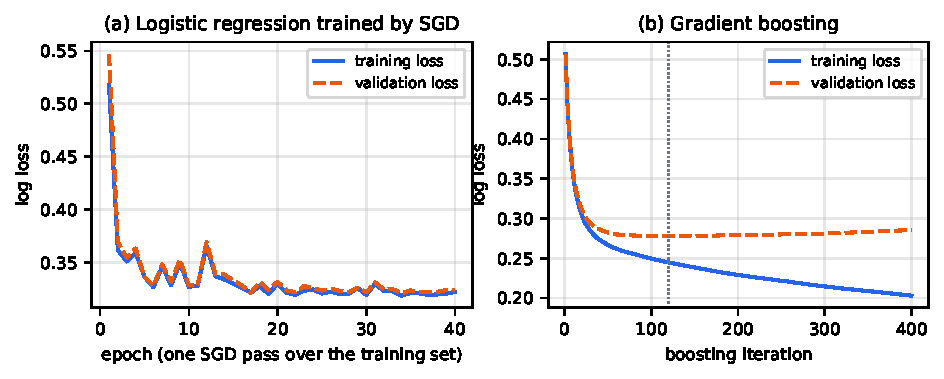
\includegraphics[width=0.95\textwidth]{loss_curve.pdf}\end{center}

\begin{itemize}
  \item \textbf{(a) Logistic regression by SGD.} \texttt{SGDClassifier(loss="log\_loss")}, one shuffled pass over the training set per epoch (\texttt{partial\_fit}), 40 epochs. Training log loss 0.518 $\to$ 0.322, validation 0.547 $\to$ 0.324, validation minimum 0.321 at epoch 34. Both curves move together $\Rightarrow$ \textbf{converged, no overfitting}. Final validation accuracy 85.5\%, same as the lbfgs solution. The wiggles early on are from the decreasing learning-rate schedule.
  \item \textbf{(b) Gradient boosting.} Log loss after each of 400 boosting iterations (\texttt{staged\_predict\_proba}, early stopping off). Training loss keeps falling to 0.203; validation loss reaches its minimum 0.278 at iteration 120 and then creeps up to 0.286. $\Rightarrow$ \textbf{mild overfitting after $\sim$120 iterations}. This agrees with cross-validation choosing 200 rather than 400 iterations.
\end{itemize}

\begin{qa}{Q: What is log loss?}
$-\frac{1}{n}\sum_i [y_i\log p_i + (1-y_i)\log(1-p_i)]$, where $p_i$ is the predicted probability of class 1. It is the quantity both logistic regression and gradient boosting (with log loss) minimize. Lower is better; 0.693 is a coin flip.
\end{qa}

\begin{qa}{Q: How do you read overfitting from these curves?}
Overfitting = training loss keeps improving while validation loss stops improving or gets worse. Plot (b) shows exactly that after iteration 120: the gap between the two curves widens. Plot (a) shows no such gap. Remedies: early stopping (stop at the validation minimum), stronger regularization, fewer/smaller trees.
\end{qa}

\begin{qa}{Q: An epoch for SGD vs an iteration for boosting --- are they comparable?}
Both are one ``step'' of an iterative optimizer: one pass over the data for SGD, one added tree for boosting. We label the axes exactly as what they are. Neither random forests nor SVMs have such a notion, which is why they have no curve.
\end{qa}

%====================================================================
\section{Fairness: the concepts}\label{sec:fairness}

For a group $g$ (e.g.\ women), true label $y$ and prediction $\yhat$:
{\small\begin{align*}
\text{Selection rate } \mathrm{SR}_g &= P(\yhat=1\mid g) && \text{how often the model says ``$>$50K''}\\
\text{True positive rate } \mathrm{TPR}_g &= P(\yhat=1\mid y=1,g) && \text{of the real high earners, share found (= recall)}\\
\text{False positive rate } \mathrm{FPR}_g &= P(\yhat=1\mid y=0,g) && \text{of the real low earners, share wrongly flagged}\\
\text{False negative rate } \mathrm{FNR}_g &= 1-\mathrm{TPR}_g\\
\text{Positive predictive value } \mathrm{PPV}_g &= P(y=1\mid \yhat=1,g) && \text{of those flagged, share truly high (= precision)}
\end{align*}}

A \textbf{gap} is the max minus the min of a rate across groups; 0 means perfectly fair under that criterion.

\begin{center}\small
\begin{tabular}{lll}
\toprule
Criterion & Requires & Gap we report \\
\midrule
Demographic (statistical) parity & equal selection rate & $\Delta_{DP}=\max_g SR_g-\min_g SR_g$ \\
Equal opportunity (Hardt et al.\ 2016) & equal TPR & $\Delta_{EO}=\max_g TPR_g-\min_g TPR_g$ \\
Equalized odds (Hardt et al.\ 2016) & equal TPR \textbf{and} equal FPR & $\Delta_{EO}$ and $\Delta_{FPR}$ \\
Predictive parity (Chouldechova 2017) & equal PPV & $\Delta_{PPV}$ \\
\bottomrule
\end{tabular}
\end{center}

\begin{qa}{Q: Explain demographic parity vs equal opportunity in plain words.}
Demographic parity: the model should approve the same \emph{fraction} of each group, regardless of the truth. Equal opportunity: among people who \emph{deserve} approval (truly $>$50K), the same fraction should be approved in each group. DP ignores the labels; EO conditions on them. DP can be criticized when base rates genuinely differ; EO is usually seen as the fairer requirement for ``merit'' decisions.
\end{qa}

\begin{qa}{Q: Why can't a model satisfy all criteria at once?}
The \textbf{impossibility theorem} (Kleinberg et al.\ 2017; Chouldechova 2017): if the base rates $P(y=1\mid g)$ differ between groups (30.4\% vs 10.9\% here) then no non-perfect classifier can have equal PPV \emph{and} equal TPR \emph{and} equal FPR. Intuition: PPV, TPR, FPR and base rate are tied together by Bayes' rule, $\mathrm{PPV}=\frac{\mathrm{TPR}\cdot p}{\mathrm{TPR}\cdot p+\mathrm{FPR}(1-p)}$; fix TPR and FPR and a different $p$ forces a different PPV. We \emph{observe} this: our unmitigated models have near-equal PPV (gap 0.03--0.07) and unequal TPR; every method that equalizes TPR/FPR blows the PPV gap up to 0.25--0.34.
\end{qa}

\begin{qa}{Q: What is ``fairness through unawareness''?}
Removing the sensitive column from the inputs. It is necessary in many legal settings but \textbf{not sufficient}: other features correlated with the sensitive attribute (proxies) let the model recover it. Our result: dropping sex and race moves the sex DP gap only from 0.181 to 0.171.
\end{qa}

\subsection{Statistical validation}
A gap computed on 12,198 test rows is itself a random quantity (a different test sample gives a slightly different gap). So:
\begin{itemize}
  \item \textbf{Bootstrap 95\% CI:} resample the test set with replacement 1,000 times, recompute the gap each time, take the 2.5th and 97.5th percentiles. Gradient boosting (without sex/race): DP 0.171 [0.158, 0.184], EO 0.075 [0.025, 0.121]. An interval that excludes 0 means significant.
  \item \textbf{Two-proportion $z$-test} on selection rates, Male vs Female: $z=\frac{\hat p_1-\hat p_2}{\sqrt{\hat p(1-\hat p)(1/n_1+1/n_2)}}$. We get $z\approx 21$--$24$ for every model, $p<10^{-10}$.
  \item \textbf{$\chi^2$ test of independence} between group and prediction (contingency table): $\chi^2>459$ by sex (1 d.o.f.), $>112$ by race (4 d.o.f.), all $p<10^{-10}$.
\end{itemize}

\begin{qa}{Q: Why bootstrap instead of a formula?}
The gap is a max-minus-min over several groups (5 races, 4 age bands), for which there is no simple closed-form standard error. Bootstrap works for any statistic. For race, the EO interval is wide ([0.08, 0.51]) because the extreme groups have only 104--116 test rows: the \emph{existence} of the gap is certain, its exact size is not.
\end{qa}

%====================================================================
\section{Results of the audit}\label{sec:results}

\subsection{By sex (gradient boosting with sex/race, test set)}
\begin{center}\small
\begin{tabular}{lrccccc}
\toprule
Group & $n$ & Sel.\ rate & TPR & FPR & PPV & Accuracy \\
\midrule
Male & 8,194 & 0.264 & 0.668 & 0.086 & 0.774 & 0.839 \\
Female & 4,004 & 0.083 & 0.577 & 0.025 & 0.725 & 0.933 \\
\midrule
Gap & & 0.181 & 0.091 & 0.060 & 0.049 & \\
\bottomrule
\end{tabular}
\end{center}
Men are selected 3.2$\times$ as often; 9 points more of the real female high earners are missed; men's FPR is 3.4$\times$ higher. \textbf{But women's accuracy is higher} --- because 90\% of women are negatives and ``predict no'' is right for them. This is the central teaching point: accuracy per group is \emph{not} a fairness metric.

\subsection{By race} Selection rate ranges from 6.0\% (Amer-Indian-Eskimo) to 28.1\% (Asian-Pac-Islander); Black 8.5\% vs White 21.8\%. Race EO gap is 0.33 with sex/race as inputs but drops to 0.13 without them: for the tiny race groups the model was using the race column almost directly (Amer-Indian-Eskimo TPR 0.33 $\to$ 0.58 after removal). So unawareness \emph{does} help rare groups.

\subsection{By age group}
\begin{center}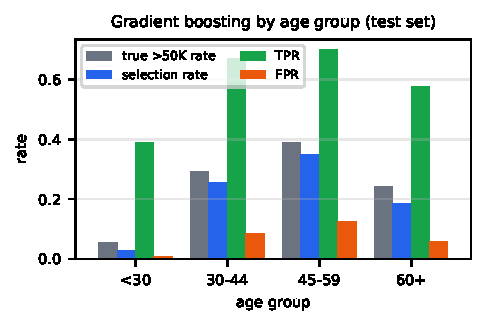
\includegraphics[width=0.55\textwidth]{age_groups.pdf}\end{center}
DP gap 0.321 (2.7\% of under-30s selected vs 34.9\% of 45--59), EO gap 0.311 (TPR 0.389 vs 0.699). The largest gaps of all. Much of it is \emph{legitimate}: the true rate is 5.4\% vs 38.8\%. But the EO gap shows the model also \emph{misses} young high earners much more often --- age acts as a strong prior.

\subsection{Intersectional (sex $\times$ race)} Among cells with $\geq$100 test rows: Asian-Pac-Islander men selected 35.5\%, Black women 4.3\% (DP 0.312). Asian-Pac-Islander women have TPR 0.40 vs 0.67 for White men. Black women have the lowest selection rate yet the highest PPV (0.79): the model is most conservative exactly where its positive predictions are most reliable.

\subsection{Ablation: with vs without sex/race} Accuracy unchanged ($\pm$0.2 points). Sex DP gap 0.181 $\to$ 0.171, EO 0.091 $\to$ 0.075. Race EO gap 0.33 $\to$ 0.13. Conclusion: proxies carry the sex bias; unawareness helps only rare groups.

\subsection{Ablation: across model families} DP gaps 0.159--0.181 for all eight models. Random forest is the fairest (DP 0.160, EO 0.073) and gradient boosting the least fair (0.181) although the most accurate. The spread (0.02) is tiny compared to the gap itself: \textbf{changing the algorithm cannot remove the bias; it comes from the data}.

%====================================================================
\section{Bias mitigation: the methods}\label{sec:mitigation}

All methods target the \textbf{sex} attribute and start from the ``without sex/race'' model. Three families:

\subsection{Pre-processing (change the data)}
\textbf{Reweighing} (Kamiran \& Calders 2012). Give each training row a weight
\[ w(g,y)=\frac{P(g)\,P(y)}{P(g,y)} \]
so that in the weighted training set group and label are independent. Our weights: high-income women 2.17, low-income women 0.85, high-income men 0.79, low-income men 1.09. The classifier is refitted with \texttt{sample\_weight}. Intuition: make the ``rare'' combination (rich woman) count more, the ``over-represented'' one (rich man) count less.

\textbf{Disparate impact remover} (Feldman et al.\ 2015). For each numeric feature, map each group's values through their within-group quantile onto the \emph{median distribution} across groups, so the feature distribution no longer reveals the group (repair level $\lambda=1$). Ranks \emph{within} a group are preserved. We repaired numeric features only (age, education-num, capital gain/loss, hours). Then retrain.

\subsection{In-processing (change the training)}
\textbf{Exponentiated-gradient reductions} (Agarwal et al.\ 2018, \texttt{fairlearn.ExponentiatedGradient}). Write the fairness requirement (DP or EO, violation $\leq\epsilon=0.01$) as linear constraints, form the Lagrangian, and solve the saddle point by alternating: the ``learner'' fits the base model on cost-sensitive (reweighted/relabelled) data, the ``adversary'' updates Lagrange multipliers with exponentiated gradient. Output: a \emph{randomized} ensemble of 12--21 base classifiers. Works with any sklearn model that accepts sample weights; we used our tuned gradient boosting and logistic regression.

\subsection{Post-processing (change the decisions)}
\textbf{Group-specific thresholds.} Keep the model's probability scores; instead of ``predict 1 if $p\geq0.5$'' use one threshold per group chosen on the \emph{validation} split so each group reaches the same TPR (the overall validation TPR at 0.5). Gradient boosting: 0.513 for men, 0.412 for women --- women need a lower score to be approved, compensating the model's under-scoring of them.

\textbf{Equalized-odds post-processing} (Hardt et al.\ 2016, \texttt{fairlearn.ThresholdOptimizer}). Finds per-group \emph{randomized} thresholds (a mixture of two thresholds) such that TPR and FPR are both equal across groups, maximizing accuracy subject to that. Fitted on validation, applied to test.

\begin{qa}{Q: Which family would you recommend in practice?}
Post-processing is the cheapest and simplest: no retraining, tiny accuracy cost (0.2 points for group thresholds), easy to explain. Its drawbacks: it needs the sensitive attribute at decision time (may be illegal) and it can hurt calibration/PPV. Pre-processing (reweighing) is attractive when you may not use the attribute at decision time. In-processing gives the strongest guarantees but is the most expensive and the hardest to explain.
\end{qa}

%====================================================================
\section{Mitigation results}

\begin{center}\small
\begin{tabular}{llcccccc}
\toprule
Model & Setting & Acc. & F1 & DP gap & EO gap & FPR gap & PPV gap \\
\midrule
\multirow{9}{*}{\shortstack[l]{Gradient\\boosting}}
 & with sex/race & 0.870 & 0.707 & 0.181 & 0.091 & 0.060 & 0.049 \\
 & without sex/race & 0.871 & 0.705 & 0.171 & 0.075 & 0.052 & 0.068 \\
 & Pre: reweighing & 0.865 & 0.684 & 0.101 & 0.098 & 0.003 & 0.185 \\
 & Pre: DI remover & 0.861 & 0.682 & 0.173 & 0.066 & 0.063 & 0.033 \\
 & In: EG (DP) & 0.847 & 0.619 & \textbf{0.023} & 0.264 & 0.045 & 0.339 \\
 & In: EG (EO) & 0.861 & 0.685 & 0.131 & 0.037 & 0.014 & 0.251 \\
 & Post: group thresholds & 0.868 & 0.701 & 0.147 & \textbf{0.002} & 0.036 & 0.133 \\
 & Post: eq.\ odds (Hardt) & 0.855 & 0.661 & 0.099 & 0.004 & 0.009 & 0.312 \\
 & reweighing + thresholds & 0.868 & 0.690 & 0.134 & 0.023 & 0.029 & 0.176 \\
\midrule
\multirow{4}{*}{\shortstack[l]{Logistic\\regression}}
 & without sex/race & 0.852 & 0.655 & 0.174 & 0.099 & 0.067 & 0.035 \\
 & Pre: reweighing & 0.842 & 0.622 & 0.083 & 0.146 & 0.007 & 0.161 \\
 & In: EG (DP) & 0.830 & 0.569 & \textbf{0.015} & 0.271 & 0.040 & 0.321 \\
 & Post: group thresholds & 0.847 & 0.644 & 0.131 & 0.036 & 0.041 & 0.105 \\
\bottomrule
\end{tabular}
\end{center}

\begin{center}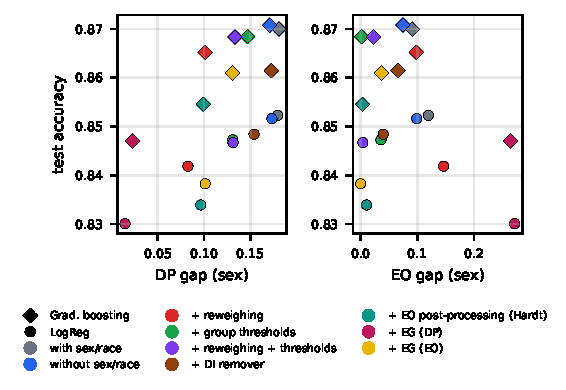
\includegraphics[width=0.6\textwidth]{tradeoff_ext.pdf}\end{center}

How to read it, method by method (gradient boosting):
\begin{itemize}
  \item \textbf{Reweighing} attacks DP: women's selection rate 8.4\% $\to$ 12\%, men's 25.5\% $\to$ 22\%, DP gap 0.171 $\to$ 0.101, FPR gap almost 0. Cost 0.6 accuracy points. EO does not improve --- it flips (women's TPR 0.69 $>$ men's 0.60) because the whole female score distribution is pushed up.
  \item \textbf{DI remover} does almost nothing (DP 0.173) because the sex proxies in this data are \emph{categorical} (relationship = Husband/Wife, marital status, occupation), which it does not repair. An honest negative result.
  \item \textbf{Group thresholds} attack EO: both sexes at TPR 0.64, EO gap 0.002, for only 0.2 accuracy points. DP improves a bit (0.147) because base rates still differ. Thresholds chosen on validation transferred cleanly to test.
  \item \textbf{Equalized-odds post-processing} equalizes TPR \emph{and} FPR (0.004 / 0.009) at 1.6 points; the price: women's FPR rises 0.026 $\to$ 0.069 and PPV gap jumps to 0.31 (men 0.81, women 0.50) --- a positive prediction for a woman becomes a coin flip.
  \item \textbf{In-processing, DP constraint} nearly closes DP (0.023) but by cutting men's selection rate to 17\% and over-correcting TPR (women 0.745 vs men 0.481, EO gap 0.264 the other way), at 2.4 accuracy and 8.6 F1 points. \textbf{EO constraint} behaves like Hardt post-processing at a smaller accuracy cost (1.0) but again PPV gap 0.25.
\end{itemize}

\begin{key}
\textbf{Take-away sentence for the viva:} ``Every method improves the criterion it targets, every improvement costs accuracy, and the strong methods pay with another criterion --- predictive parity --- exactly as the impossibility theorem predicts. On this task the simple group thresholds are the best accuracy-per-fairness deal for equal opportunity, and reweighing for demographic parity.''
\end{key}

%====================================================================
\section{Experimental setup facts}
\begin{itemize}
  \item Hardware: Apple M4 laptop CPU, 16 GB RAM. Full pipeline $\approx$95 s + extensions $\approx$90 s. Also runs on free Google Colab.
  \item Software: Python 3.12.13, scikit-learn 1.9.1, fairlearn 0.15.0, NumPy 2.5.4, pandas 3.1.1, SciPy 1.18.1, Matplotlib 3.11.
  \item Seed 42 for the split, the models, the bootstrap, SGD shuffling and the randomized post-processors.
  \item Code: \texttt{experiments/run\_experiments.py} (part 1), \texttt{experiments/run\_extensions.py} (part 2), identical Colab notebook in \texttt{notebooks/}. All CSV/JSON outputs in \texttt{experiments/results/}. \texttt{check\_report\_numbers.py} verifies that 143 numbers in the report match the CSVs.
\end{itemize}

%====================================================================
\section{Limitations we admit (say them before the examiner does)}
\begin{enumerate}
  \item One dataset, 1994 US census: findings describe that data, not today's population (Ding et al.\ 2021 propose newer ``folktables'' data).
  \item Sex is binary in the data; three race groups have only $\sim$100 test rows; some intersectional cells have 34--73 rows, so their estimates are noisy.
  \item Mitigation targeted sex only; race and age gaps of the mitigated models are essentially unchanged.
  \item Our disparate impact remover repairs numeric columns only.
  \item All post- and in-processing rules use the sensitive attribute at decision time, which is not permitted in every legal setting.
  \item Not done from the proposal: Prejudice Remover (we used the Agarwal reductions instead, which the proposal listed as the alternative) and the German Credit dataset.
  \item Experiments ran on a laptop rather than on Colab; the code is identical.
\end{enumerate}

%====================================================================
\section{Likely viva questions, quick answers}\label{sec:questions}

\begin{qa}{Why classical models and not deep learning?}
Course rule, and realistic: in finance, logistic regression and tree ensembles are the standard because they are interpretable and accepted by regulators. On tabular data of this size they are also as accurate as neural nets.
\end{qa}
\begin{qa}{How did you choose hyperparameters?}
Grid search with 3-fold stratified cross-validation on the training split, scoring F1. The test set was never used for any choice.
\end{qa}
\begin{qa}{Why F1 and not accuracy for model selection?}
With 76\% negatives, a model predicting ``no'' for everyone is 76\% accurate. F1 balances precision and recall on the minority class we care about.
\end{qa}
\begin{qa}{Isn't the gap just because women really earn less in the data?}
Partly, and that is why we report several criteria. Demographic parity compares to nothing; equal opportunity compares only among true high earners, and there the model still finds 9 points fewer women (and 31 points fewer under-30s). That part cannot be explained by base rates.
\end{qa}
\begin{qa}{You removed sex and race; why is the model still biased?}
Proxies. Relationship (Husband/Wife) is almost a sex label; marital status, occupation and hours per week are strongly correlated with sex. The model reconstructs the attribute from them.
\end{qa}
\begin{qa}{What is a bootstrap confidence interval?}
Resample the test set with replacement many times, recompute the statistic each time, take the 2.5 and 97.5 percentiles. It estimates how much the statistic would vary with a different test sample.
\end{qa}
\begin{qa}{What does $p<10^{-10}$ mean here?}
If the model were selecting men and women at the same rate, the chance of seeing a difference this large in 12,198 rows is less than one in ten billion. The gap is not sampling noise.
\end{qa}
\begin{qa}{What is the accuracy--fairness trade-off?}
Every mitigation that reduced a gap also reduced accuracy (0.2 to 2.4 points). Fig.~4 in the report shows that no mitigated point lies above the unmitigated one. The size of the cost depends on the method and the criterion.
\end{qa}
\begin{qa}{Which result surprised you?}
That the disparate impact remover did almost nothing, and that equalizing TPR/FPR made positive predictions for women much less reliable (PPV 0.50). Both are explained after the fact (categorical proxies; impossibility theorem), but they show that mitigation must be audited too.
\end{qa}
\begin{qa}{How would you deploy this?}
Audit first (per-group rates + CIs), pick the criterion the application needs (EO for merit decisions, DP where equal access is the goal), apply the cheapest method that meets it (thresholds or reweighing), and re-audit all criteria including the ones not targeted. Document everything.
\end{qa}
\begin{qa}{What would you do with more time?}
Mitigate several attributes jointly, a repair method that handles categorical proxies, intersectional groups with small-sample corrections, repeat over several random splits to get CIs on the trade-off itself, and the newer folktables census data.
\end{qa}

\end{document}
